\documentclass[10pt,aspectratio=169,handout]{beamer}

\usepackage[utf8]{inputenc}
\usepackage[ngerman]{babel}
\usepackage{utopia}
\usetheme{Darmstadt}
\usecolortheme{default}
\usepackage{xcolor}
\usepackage{graphicx}
\usepackage{amsmath}
\usepackage{amsthm}
\usepackage{amssymb}
\usepackage{amsfonts}
\usepackage{mathtools}
\usepackage{dsfont}
\usepackage{hyperref}
\usepackage[most]{tcolorbox}
\usepackage{tikz}
\usepackage{adjustbox}
\usepackage{mathrsfs}
\usepackage{minted}
\usetikzlibrary{cd}
\usetikzlibrary{positioning}
\usetikzlibrary{calc}
\usetikzlibrary{arrows.meta}
\setbeamertemplate{theorems}[numbered]
\setbeamertemplate{navigation symbols}{}
\newtranslation[to=ngerman]{Theorem}{Satz}
\def\C{\mathbb{C}}
\def\R{\mathbb{R}}
\def\Q{\mathbb{Q}}
\def\N{\mathbb{N}}
\def\Z{\mathbb{Z}}
\def\cA{\mathcal{A}}
\definecolor{LightGray}{gray}{0.9}


\begin{document}

\title{Principles of Machine Learning: Exercise 1}
\date{06.11.2023}
\author{Alina Pollehn (3197257), Julian Litz (3362592), Manuel Hinz (3334548)\\
    Felix Göhde (3336445), Felix Lehmann (3177181), Caspar Wiswesser (3221493)\\
    Adrian Köring (3347785), Greta Günther (3326765), Linus Mallwitz (3327653)\\
    Niklas Mueller-Goldingen (3363219), Jennifer Kroppen (???????)}

\begin{frame}
    \maketitle
\end{frame}

\section{Exercise 1.2}

% \begin{frame}
%     \frametitle{test}
%     %\inputminted[bgcolor=LightGray]{python}{tmp.py}
% \end{frame}

\begin{frame}
    \frametitle{Task 1.2.0}
    \begin{itemize}
        \item Given the following two rule sets, implement code that solves the least squares problem between $X^T$ and $y$.
        \item Afterwards the code should calculate $\hat{y}$ using the calculated weights.
    \end{itemize}
\end{frame}

\begin{frame}
    \frametitle{Task 1.2.0}
    \begin{minipage}{0.45\textwidth}
        \begin{table}[]
            \caption[short]{Rule 110}
            \begin{tabular}{llll}
                \hline
                     & $X^T$ &      & y    \\ \hline
                $+1$ & $+1$  & $+1$ & $+1$ \\
                $+1$ & $+1$  & $-1$ & $-1$ \\
                $+1$ & $-1$  & $+1$ & $-1$ \\
                $+1$ & $-1$  & $-1$ & $-1$ \\
                $-1$ & $+1$  & $+1$ & $+1$ \\
                $-1$ & $+1$  & $-1$ & $-1$ \\
                $-1$ & $-1$  & $+1$ & $-1$ \\
                $-1$ & $-1$  & $-1$ & $+1$ \\ \hline
            \end{tabular}
        \end{table}
    \end{minipage}
    \begin{minipage}{0.45\textwidth}
        \begin{table}[]
            \caption[short]{Rule 126}
            \begin{tabular}{llll}
                \hline
                     & $X^T$ &      & y    \\ \hline
                $+1$ & $+1$  & $+1$ & $+1$ \\
                $+1$ & $+1$  & $-1$ & $-1$ \\
                $+1$ & $-1$  & $+1$ & $-1$ \\
                $+1$ & $-1$  & $-1$ & $-1$ \\
                $-1$ & $+1$  & $+1$ & $-1$ \\
                $-1$ & $+1$  & $-1$ & $-1$ \\
                $-1$ & $-1$  & $+1$ & $-1$ \\
                $-1$ & $-1$  & $-1$ & $+1$ \\ \hline
            \end{tabular}
        \end{table}
    \end{minipage}
\end{frame}

\begin{frame}
    \frametitle{Task 1.2.1}
    \inputminted[bgcolor=LightGray,fontsize=\small]{python}{calcyhat.py}
    \begin{minipage}{0.45\textwidth}
        $\hat{y}_{110}= \begin{pmatrix}
                +0.25 \\
                -0.25 \\
                -0.25 \\
                -0.75 \\
                +0.75 \\
                +0.25 \\
                +0.25 \\
                -0.25 \\
            \end{pmatrix}$
    \end{minipage}
    \begin{minipage}{0.45\textwidth}
        $\hat{y}_{126}= \begin{pmatrix}
                +1.57e-16 \\
                -1.23e-32 \\
                +1.57e-16 \\
                -1.23e-32 \\
                +1.23e-32 \\
                -1.57e-16 \\
                +1.23e-32 \\
                -1.57e-16 \\
            \end{pmatrix}$
    \end{minipage}
\end{frame}

\begin{frame}
    \frametitle{Task 1.2.1}
    \begin{itemize}
        \item The first calculation is numerically stable
        \item Even though the difference between the two rulesets is only one number, the second calculation becomes numerically unstable
    \end{itemize}
\end{frame}

\begin{frame}
    \frametitle{Task 1.2.2}
    Implement a function phi which takes a vector $x$ with $n$ elements and realizes the following transformation:
    $\varphi : \{+1, -1\}^n \to \{+1, -1\}^{2^n} $
    \inputminted[bgcolor=LightGray,fontsize=\small]{python}{phi.py}
\end{frame}

\begin{frame}
    \frametitle{Task 1.2.3}
    Given the previously introduced function phi we compute the matrix
    $\phi^T = \begin{bmatrix}
            \rule[.5ex]{2.5ex}{0.5pt} & \varphi^T_0 & \rule[.5ex]{2.5ex}{0.5pt} \\
            \rule[.5ex]{2.5ex}{0.5pt} & \varphi^T_1 & \rule[.5ex]{2.5ex}{0.5pt} \\
                                      & \vdots      &                           \\
            \rule[.5ex]{2.5ex}{0.5pt} & \varphi^T_7 & \rule[.5ex]{2.5ex}{0.5pt} \\
        \end{bmatrix}$
    Solve the least squares problem between $\phi^T$ and $y$ and calculate $\hat{y}$ using the calculated weights.
    \inputminted[bgcolor=LightGray,fontsize=\small]{python}{matrixphi.py}
\end{frame}

\begin{frame}
    \frametitle{Task 1.2.3}
    \begin{minipage}{0.45\textwidth}
        $\hat{y}_{110}= \begin{pmatrix}
                +1 \\
                -1 \\
                -1 \\
                -1 \\
                +1 \\
                -1 \\
                -1 \\
                +1
            \end{pmatrix}$
    \end{minipage}
    \begin{minipage}{0.45\textwidth}
        $\hat{y}_{126}= \begin{pmatrix}
                +1 \\
                -1 \\
                -1 \\
                -1 \\
                -1 \\
                -1 \\
                -1 \\
                +1
            \end{pmatrix}$
    \end{minipage}
    
    \vspace{1cm}
    We now observe that $\hat{y}_{110}=y_{110}$ and $\hat{y}_{126}=y_{126}$.
    We "trained" our "parameters" w with all possible inputs/"data" to archieve an output as close as possible to our rule so that we get a good output according to our rule for every input. We had to pay the price of computing a high dimensional feature map Phi. Because of this our "training" aka. the search for the least squares solution is highly complex (in contrast to the computing of the rule once the parameters have been found)
\end{frame}

\section{Exercise 1.3}

\begin{frame}
    \frametitle{Fractal dimensions}

    \begin{enumerate}
        \item Binarize the image
        \item Partition the image into $2^l$ boxes for $l=1,\dots,L-2$,
        \item Calculate the fractal dimension using linear regression \[D\cdot \log\left(\frac{1}{s_l}\right)+b=\log(n_l)\]
    \end{enumerate}
    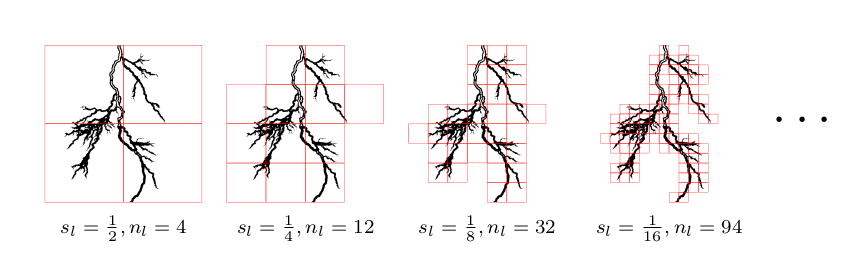
\includegraphics[scale=0.4]{images/boxes.png}

\end{frame}

\begin{frame}
    \frametitle{Implementation: Box counting}
    \inputminted[bgcolor=LightGray,fontsize=\small]{python}{box_counting.py}
\end{frame}

\begin{frame}
    \frametitle{Implementation: Calculating the fractal dimension}
    \inputminted[bgcolor=LightGray,fontsize=\small]{python}{get_slope.py}
    where np.vander generates the Vandermonde matrix
    \[V=\begin{bmatrix}
            1      & \log(2^1)^1     \\
            1      & \log(2^2)^1     \\
            \vdots & \vdots          \\
            1      & \log(2^{L-2})^1
        \end{bmatrix}\]
\end{frame}

\begin{frame}
    \frametitle{Results}

    \begin{minipage}{0.45\textwidth}
        \begin{enumerate}
            \item Fractal dimension\begin{itemize}
                      \item Tree: $\approx 1.846$
                      \item Lighting: $\approx1.493$
                  \end{itemize}
            \item The fractal dimension of the image ``lighting.png'' is higher
        \end{enumerate}
    \end{minipage}
    \begin{minipage}{0.45\textwidth}
        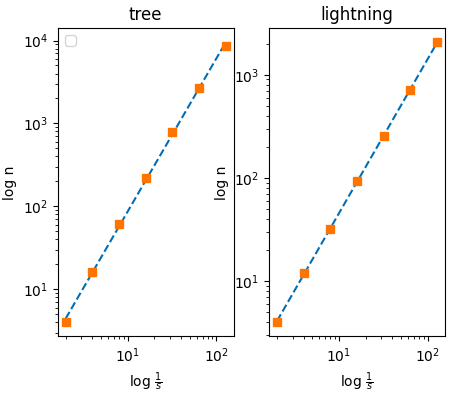
\includegraphics[scale=0.4]{images/plots.png}
    \end{minipage}
\end{frame}

\begin{frame}
    \frametitle{Learnings}
    \begin{enumerate}
        \item Fractal dimensions
        \item Fractal dimensions as a least squares problem using box counting
        \item Application of least squares to a wider class of problems
    \end{enumerate}
\end{frame}

\end{document}
